\section{Kódolási alapismeretek}

A nagyobb nyílt forrású projektek a kódolás, kódszervezés során egy meghatározott konvenciót követnek, bár egy olyan méretű projekt esetén, mint a \textit{GNOME} az egyes részterületeken lehetnek eltérések, azzal együtt is, hogy az azonosságok nyilván erős többségben vannak. Lássuk mik ezek a \textit{GNOME}, illetve a \textit{GTK} projektek esetén.

\subsection{Forráskód formázása}

A \textit{GTK} fejlesztői a \textit{GNU coding standard}\cite{gnucodingstandards}, illetve a \textit{Linux kernel coding style}\cite{linuxcodingstyle} irányelveit alkalmazzák, ami mindaddig nem bír különösebb jelentőséggel, amíg nem áll szándékunkban a \textit{GTK} fejlesztésébe, javításába belefogni, ugyanakkor két oknál fogva mégis érdemes megemlíteni. Ha még nem ismerkedtünk meg egyetlen kódolási konvencióval sem, akkor az említett kettő -- mind népszerűségük, mind letisztult mivoltuk okán -- alkalmas választás lehet. A másik ok, hogy néhány a fejlesztés során hasznos információ ezen konvenciókból következik.

\subsection{Elnevezési konvenciók}
 \index{GTK@\textit{GTK}!kódolási konvenciók}
 \index{GTK@\textit{GTK}!kódolási konvenciók!formázás}
 \index{GTK@\textit{GTK}!kódolási konvenciók!nevezéktan}

A \textit{GNOME} projekten belül nem csak formázási, de elnevezési konvenciók is életben vannak. Ezek az egyes funkciót megvalósító szoftverelemekre (pl: függvények, makrók, \dots) vonatkoznak, melyek közül a az alábbiak már a legegyszerűbb példák esetén is feltűnnek.

\begin{itemize}
  \item az egyes nevek részekre oszthatóak,
  \item a részek meghatározott sorrendben követik egymást, ahol
  \begin{itemize}
    \item kezdve a \textit{GNOME} megfelelő projektjével (pl: \texttt{atk}, \texttt{gtk}, \dots),
    \item folytatva a vonatkozó osztály nevével (pl: \texttt{entry}, \texttt{label}, \dots),
    \item befejezve a megvalósított művelettel (pl: \texttt{get}, \texttt{set}, \dots),
    \item illetve a művelet tárgyával (pl: \texttt{text}, \texttt{value}, \dots),
  \end{itemize}
  \item a részeket aláhúzásjel ('\texttt{\_}') választja el,
  \item az egyes részek rendszerint vagy csak kis-, vagy csak nagybetűket, illetve számokat tartalmaznak.
\end{itemize}

Fentieknek megfelelően egy -- a \textit{GTK+} által implementált -- rádiógomb aktív mivoltát lekérdező függvény neve a \texttt{gtk} prefixszel kezdődik, amit a osztálynévként a \texttt{radio\_button} követ, majd lekérdezésről lévén szó \texttt{get} követ, végül pedig a tulajdonság neve következik (\texttt{actvie}). Aláhúzás jelekkel összefűzve tehát \texttt{gtk\_radio\_button\_get\_active}.

A \textit{C++}, illetve a \textit{Python} nyelvű változatok esetén is hasonló az elnevezés módszertana a nyelvből fakadó sajátosságok okozta eltéréssel természetesen. A \textit{gtkmm} esetén a projektek nevét tartalmazó prefix szerepét a \textit{Gtk} névtér veszi át, míg az osztályok neve a \textit{C++} osztályok neve lesz, melyek tagfüggvényei az előbbi két előtag (pl: \texttt{gtk\_entry}) nélküli nevel lesznek (pl: \texttt{set\_text}). A \textit{PyGobject} esetén a névtér szerepét a \textit{Gtk} modul veszi át, az osztályokét pedig a megfelelő \textit{Python} objektumok.

\subsection{Fejlécfájlok és importálás}
 \index{GTK@\textit{GTK}!fejlécfájlok}

Szakítva az előző főverziónál (\textit{2.x}) megszokottaktól \textit{GTK+} verziótól, a \textit{C}, illetve a \textit{C++} változat egyaránt csak egyetlen állomány beszerkesztésére (\textit{include}) van lehetőség és szükség. A korábbiakban az egyes \textit{widget}ekhez tartozó fejlécállományok (pl: \texttt{gtk/gtkentry.h}) beszerkesztésére külön-külön volt lehetőség függően attól, melyekre van, illetve melyekre nincs szükség. Most azonban közvetlenül csak a \texttt{gtk/gtk.h} szerkeszthető be, a többi fejlécállomány esetén hibaüzenetet kapunk. Így mind a \textit{C}, mind a \textit{C++} változat azonos módon működik, ami egyébiránt hasonlít a \textit{Python} modul importjára.

\section{Minimálisan alkalmazás}
\label{sec:gtkminimal}
\label{sec:gtkmmminimal}

Ennyi bevezető után lássuk egymás mellett (\ref{lst:gtkminimal}. Kódrészlet) a három nyelvi változat (\textit{C}, \textit{C++}, illetve \textit{Python}) kódját számba véve azok hasonlóságait és különbözőségeit. Ami talán első látásra is feltűnő, hogy messze a \textit{GTK+} változat ''kódsűrűsége'' a legnagyobb, vagyis a \textit{C} nyelvű változat igényli ugyanazon funkcionalitás mellett a legtöbb kódsor (\ref{gtkminimalc:end} sor) begépelését, következésképp a legtöbb munkát is. Ez persze nem jelenthet különösebb meglepetést ha van némi tapasztalatunk az interpretált, illetve a fordított, a procedurális, illetve az objektum központú nyelvek esetén elérhető fejlesztési sebesség terén.

\subsection{Forráskód}

\lsttriplesource
{sources/gtk_minimal.c}
{sources/gtk_minimal.cc}
{sources/gtk_minimal.py}
{Minimálisan szükséges kód \textit{GTK+}, \textit{gtkmm}, illetve \textit{PyGobject} használata mellett}
{lst:gtkminimal}

Első közelítésben a már említett formai különbségek lehetnek szembeötlőek, ugyanakkor számos, a tartalmat, megvalósítást érintő eltérés is felfedezhető ebben a még oly kevést kódsort tartalmazó példában. Ezek megértése nagyban könnyíti az egyes nyelvi változatok közötti átjárást és ne utolsó sorban a \textit{GTK} koncepcionális sajátosságaira is rávilágít. Lássuk tehát sorról sorra az imént olvasott kódok magyarázatát.

\begin{enumerate}
 \index{GTK@\textit{GTK}!fejlécfájlok}
 \item[\ref{gtkminimalc:include}. sor] A \textit{header} fájlok beszerkesztésének különbözőségeiről az előzőekben esett szó, így erre itt csak azt megemlítendő térünk ki, hogy a \textit{Python} változat \texttt{import} parancsának azt a változatát alkalmazzuk, ami azt legerősebb hasonlóságot eredményezi a másik két nyelvi változattal, már ami a \texttt{gtk} kulcsszó forráskódban történő megjelenéseinek helyét illeti.

 \item[\ref{gtkminimalc:main}. sor] Ez a sor a programjaink belépési pontja, azaz itt kezdődik meg a futtatás, már legalábbis ami a \textit{C}/\textit{C++} változatot illeti. A \textit{Python} nyelv esetén az \texttt{import} parancs már végrehajtásra került mire ide jutunk, sőt erre a kódsorra voltaképpen nincs is feltétlenül szükséges\cite[fej.~27.4.]{pythonlib}, leginkább csak a másik két példához való még erősebb hasonlóság végett került be ez a kódsor. Fontossá a \texttt{main} függvények tulajdonképpen csak a parancssori paraméterek \textit{GTK}-nak történő átadás\ref{gtkminimalc:gtkmain} szempontjából válnak.

 \item[\ref{gtkminimalc:windowdeclare}. sor] A \textit{C} nyelvi verzióban kénytelenek vagyunk blokk elején deklarálni azt a változót -- ami ez esetben \textit{widget}ünk címét tartalmazza majd -- mivel az \textit{ISO C90} szabvány még nem, majd csak az \textit{ISO C99} támogatja a blokkon belül kifejezés után elhelyezett változó deklarációkat. Ezt viszont sem \textit{3.0}-nál korábbi \textit{GCC}, sem pedig a \textit{Microsoft Visual Studio} \textit{C} fordítója nem támogatja, vagyis problémába ütköznénk a \textit{C++} példában használt módszerrel, így a biztonság kedvéért maradunk a hagyományoknál, azaz lokális változók deklarációja csak blokkok kezdetén szerepel.

 \index{Main@\texttt{Main}}
 \index{Gtk@\texttt{Gtk}!függvények!init@\texttt{init}}
 \item[\ref{gtkminimalc:gtkmain}. sor] Eljutottunk végre az első \textit{GTK} specifikus híváshoz, mely a \textit{Python} változatból teljesen hiányzik, míg a \textit{C}, illetve a \textit{C++} verzióban funkciójuk azonos, mégis van köztük árnyalatnyi különbség. A \textit{GTK+} esetén az \texttt{argc}, valamint az \texttt{argv} változók címeit adjuk át, biztosítandó, hogy az \textit{init} függvény a \textit{GTK}-nak szóló paramétereket\footnote{a \textit{GTK} által értelmezett parancssori paramétereket összefoglalója \href{http://library.gnome.org/devel/gtk/stable/gtk-running.html}{itt} olvassható.} el tudja távolítani a tömbből és azok számával csökkenteni tudja \texttt{argc} értékét. Erre a \textit{C++}-os változat esetén a cím szerinti átadásra azért nincs szükség, mert -- még ha nem is látszik -- mindkét változóra referencia adódik át a \texttt{Gtk::Main} konstruktorának. A \textit{Python} változat esetén nincs \texttt{init} jellegű függvényhívás, mivel az inicializálás a modul (\textit{gi.repository.Gtk}) importálásával implicit módon megtörténik, másrészről a parancssori paraméterek a \textit{sys} modulon keresztül bárhol hozzáférhetőek, azok paraméterként való átadási így felesleges.

 \index{GtkWindow@\texttt{GtkWindow}!függvények!new@\texttt{new}}
 \item[\ref{gtkminimalcc:windowdeclare}. sor] Első \textit{widget}ünk létrehozása a már említett nevezéktan szerinti függvények meghívásával történik. Minden \textit{widget}típushoz létezik egy mondjuk úgy konstruktor, melyet meghívva egy új -- az adott típushoz tartozó -- \textit{widget}et kapunk vissza. A hívás mikéntje természetesen függ a nyelvtől magától, illetve attól is, hogy a nyelv esetén használható-e, illetve használjuk-e az objektumok-orientált megközelítést. A \textit{C} nyelvi változat esetén a \texttt{gtk\_widgetnév\_new} forma használatos, addig a \textit{C++} esetében a prefixek szerepét a névterek veszik át, tehát általános formában a \texttt{Gtk::WidgetNév::WidgetNév} írható le a konstruktor. A \textit{Python} szintén névterekkel operál, ahol azok határait a modulok jelentik, melyek neveit egymástól, illetve függvényeiktől pont (\texttt{.}) választja el, vagyis a konstruktor \texttt{Gtk.WidgetNév} formában írhatóak le.

\index{lebegő referencia@''lebegő'' referencia}
A különbség nem is annyira a nevekben, mint inkább a memória kezelésében rejlik, hiszen egy újólag létrehozott objektum felszabadításáról \textit{C} esetén magunknak kell gondoskodnunk, míg a \textit{C++} a tőle megszokott módon felszabadítja a lokális változókat. Ugyanakkor érdemes itt visszautalni a már említett referencia számlálásra, illetve a ''lebegő'' referenciára, melyek révén a különböző nyelvi változat esetén mód van arra, hogy csak a legfelső szintű elemről kelljen ebben a tekintetben magunknak gondoskodnunk, a \textit{GTK} a többi elem memóriakezelését maga menedzseli.

Az ablak létrehozásában meg egy különbség fedezhető fel a \textit{C}, illetve a másik két változat kötött, mégpedig a paraméterkezelés kapcsán. Előbbi esetben meg kell mondanunk az ablak típusát (toplevel) -- hiszen a \textit{C} nyelv nem tesz lehetővé a paraméterek esetén alapértelmezett értékét --, míg a másik két esetben erre nincs szükség. Ez a paraméter ugyan mindkét esetben létezik és ki is írható, ugyanakkor alapértelmezett értékük pont az, amit a \textit{C} változat esetén kiírtunk.

 \index{widget@\textit{widget}!szignálok!delete-event@\texttt{delete-event}}
 \index{Main@\texttt{Main}!függvények!run@\texttt{quit}}
 \item[\ref{gtkminimalc:windowdelete}. sor] Anélkül, hogy a szignálok kezelésének rejtelmeiben elmerülnénk egy gondolatnyi kitérőt érdemes ezen kódsor a kapcsán tenni. Elsőként azt érdemes tisztázni mire szolgál a \texttt{delete-event} szignál. Ez a szignál akkor váltódik ki, amikor az ablakunk felhasználó interakció hatására bezáródik. Ez számos interakciót jelenthet -- operációs rendszertől és ablakkezelőtől függően --, de alapvetően az ablak jobb felső sarkában\footnote{\textit{Mac OS X}, illetve az újabb \textit{Ubuntu} verziók esetén bal felső sarok} lévő \textit{X} gomb, vagy az \texttt{Alt+F4} billentyűk lenyomására kell gondolnunk.

A \textit{C}, illetve a \textit{Python} nyelvű változat ezen esemény bekövetkeztekor a \textit{GTK} főciklusát szeretné leállítani, ami annak révén ér el, hogy a \texttt{delete-event} szignálra a nyelvi változatnak megfelelő \texttt{main\_quit} függvényt köti fel. Figyelembe véve, hogy a \texttt{delete-event} alapértelmezett szignálkezelője megszünteti (\textit{destroy}) az ablakot, ez az eljárás logikus, lévén egy programnak főablak nélkül nincs igazán sok értelme. A \textit{C++} változat viszont ugyanebben a tekintetben látszólag semmilyen lépést sem tesz, ugyanakkor a megfigyelhetjük, hogy néhány sorral lejjebb (\ref{gtkminimalc:gtkrun}. sor) a \texttt{run} függvények paraméterként átadja az ablakot, ami nagyon hasonló eredményre vezet. Egészen pontosan nem csak az átadott ablak megszűnésekor, de az eltüntetésekor (\textit{hide}) is ki fog lépni a főciklus.

 \index{GtkWidget@\texttt{GtkWidget}!függvények!show@\texttt{show}}
 \item[\ref{gtkminimalc:windowshow}. sor] Ezek után nem érhet meglepetésként bennünket, hogy miért nincs szükség a \textit{C++} változat esetén az megjelenítő függvény meghívására, ezt az átadott ablakra a főciklust elindító \texttt{run} függvény megteszi, ami logikus is hiszen ha nincs egyetlen látható ablakunk sem, akkor nehéz olyan felhasználó interakció kezdeményezni -- legalábbis a felhasználói felületen keresztül --, ami a főciklus kilépését eredményezné.

 \index{Main@\texttt{Main}!függvények!run@\texttt{run}}
 \index{Gtk@\texttt{Gtk}!függvények!main@\texttt{main}}
 \item[\ref{gtkminimalc:gtkrun}. sor] A hívások a -- korábban már részletezett -- \textit{GTK main loop}ot indítják, azaz itt kezdődik meg az az eseményvezérelt szakasz, mely a választott nyelvtől függően a \texttt{gtk\_main\_quit}, a \texttt{Gtk::Main::quit}, vagy a \texttt{Gtk.main\_quit} meghívásáig tart. Ezekben a minimális példákban erre az egyetlen mód a futtatáskor megjelenő ablak bezárása, hiszen az imént említett függvényeket az ennek hatására kiváltódó \texttt{delete-event} szignálhoz rendeltük.  Miután a szignált ''kezelő'' függvény lefutott a \textit{GTK} főciklusa (\textit{main loop}) kilép, azaz a \texttt{run} függvény futása befejeződik, a program futtatása az azt követő soron folytatódhat.

 \item[\ref{gtkminimalc:return}. sor] Visszatérési értékünk mindhárom esetben 0, amit a rendelkezésre álló nyelvi módszerek legegyszerűbbikével érünk el, ezzel jelezvén a hívó félnek, hogy a futás rendben lezajlott.
\end{enumerate}

\subsection{Fordítás és futtatás}
\index{fordítás}
\index{futtatás}

A korábbiakban már említett metodika mellet a mostani forráskódok\footnote{természetesen csak a \textit{C}, illetve a \textit{C++} változat fordítandó a \textit{Python} nem} fordítása a követlezőképp néz ki:

\lstcompiles
{gtk_minimal.c}{gtk_minimal}
{gtkmm_minimal.cc}{gtkmm_minimal}

A futtatás tekintetében próbálkozzunk a \texttt{./gtk\_minimal}, illetve a \texttt{./gtkmm\_minimal}, illetve a \texttt{python3 gtk\_minimal.py} parancsokkal abban a könyvtárban, ahol a forrásállományaink is találhatóak.

\subsection{Eredmény}

Nagy meglepetést nem várhatunk egy ilyen méretű applikációtól, viszont az azért kell tudnunk értékelni, hogy a legrosszabb esetben is alig másfél tucat kódsorból egy működő grafikus felhasználó felületet lehet létrehozni, melynek eredménye az alábbi képeken látható.


\begin{figure}[ht]
\begin{center}
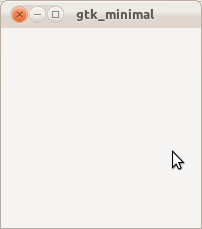
\includegraphics[height=40mm]{images/screenshot_gtk_minimal.png}\hspace{0.05\textwidth}
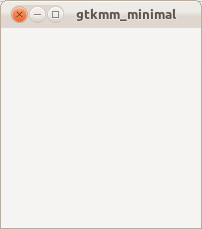
\includegraphics[height=40mm]{images/screenshot_gtkmm_minimal.png}\hspace{0.05\textwidth}
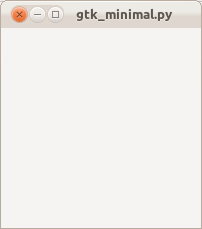
\includegraphics[height=40mm]{images/screenshot_gtkpy_minimal.png}
\caption{Minimális mintapéldák képernyőképi}{\textit{C}, \textit{C++}, \textit{Python} változat}
\label{fig:screenshotminimap}
\end{center}
\end{figure}

\index{widget@\textit{widget}!szignálok!delete-event@\texttt{delete-event}}
\index{ablakkezelő}
\index{ablakkezelő!bezárás}
\index{ablakkezelő!minimalizálás}
\index{ablakkezelő!minimalizálás}
Tulajdonképpen csak egy puszta ablakot kapunk, bármilyen gomb, vagy egyéb elem nélkül. Minden díszítés -- az ablak fejléce, a címsor szövege, a minimalizáló, maximalizáló és a bezáró gombok -- egyaránt az ablakkezelőnek és nem a \textit{GTK}-nak köszönhetőek. Ez utóbbi gombhoz kötődik az egyetlen \textit{GTK} szempontjából is érdemleges\footnote{a minimalizálása és a maximalizálás az ablakkezelő hatáskörébe tartoznak} művelet, ami a már több ízben is említett \texttt{delete-event} szignált fogja kiváltani, ami a végső soron a program futásának befejezéséhez vezet.

\section{Tesztelés}

Elsőre talán azt gondolhatjuk, hogy a fenti ablakon igazán nincs mit tesztelni, egy feladat mégis akad, mégpedig az, hogy a futó applikációt, illetve annak egyetlen ablakát megtaláljuk, majd bezárjuk, ami mint látni fogjuk azért jelent némi feladatot.

\subsection{Forráskód}

\index{Dogtail@\textit{Dogtail}!tree@\texttt{tree}}
\index{Dogtail@\textit{Dogtail}!procedural@\texttt{procedural}}
Az ablakok tesztelésére szolgáló tesztek forráskódjai (\ref{lst:dogtailminimal}. Kódrészlet) mindössze két sorban térnek el egymástól, ami a gyakorlatban nem jelent érdemi különbséget, ugyanakkor rámutat arra, hogy a \textit{Dogtail} használatával két API is rendelkezésünkre áll az applikációk teszteléséhez. Ezek a már említett \textit{tree}, illetve a \texttt{procedural} API. Előbbi egy objektumorinentált megközelítést alkalmazva teszi lehetővé, hogy a felhasználó felület egyes elemeit -- gombok, ablakok, menük -- elérjük, azokon műveleteket végezzünk, illetve a köztük fennálló összefüggéseket feltárjuk. Utóbbi az ablakokra, illetve azok elemeire -- melyeket nevükkel hivatkozhatunk -- ad fókuszt, illetve végez egyéb műveleteket, aminek révén egyszerűen vezérelhetjük a tesztelendő alkalmazást.

\index{Python@\textit{Python}!unittest@\texttt{unittest}}
A következő kód -- a fejlesztési példától némiképpen eltérően -- nem szorítkozik a minimálisan szükséges kódsorok ismertetésére, ennél egy kicsit tovább megy. Ennek oka kettős: egyrészről a minimálisan alig néhány sorra van szükség, másrészről igyekszünk egy, a valós életben is használható kóddal szolgálni, aminek része egy tesztelési kertrendszer (framework), ebben az esetben a \textit{Python} \textit{unittest} modulja. Nem mellesleg a \textit{Dogtail} saját tesztjei is ezt a modult alkalmazzák, a következőkben ismertetettekhez nagyon hasonló esetenként teljesen azonos módon. Ahogy a korábbiakban, úgy itt sem ismertetjük a nyelvi eszközökből adódó sajátosságokat, hacsak annak nincs kifejezett hatása a tesztelésre, így a \texttt{unittest} modul is csak olyan mértékben kerül ismertetésre, amennyire az a megértés szempontjából szükséges. Tesztelendő alkalmazásnak a \textit{GTK} demó alkalmazását választottuk, mely minden alapvető \textit{widget}re tartalmaz példát és része azon fejlestői korábban már említett csomagnak, mely a \textit{C} nyelvű fordításhoz szükséges.

\lstdoublepysource
{sources/dogtail_minimal_procedural.py}
{sources/dogtail_minimal_tree.py}
{Minimálisan szükséges teszt \textit{tree}, illetve \textit{procedural} API használata mellett}
{lst:dogtailminimal}

\begin{enumerate}
 \item[\ref{dogtailminimal:importtree}. sor] A két különbözőséget adó sor egyike, ahol az \textit{Dogtail} előbbiekben említett \texttt{procedural}, illetve \texttt{tree} moduljait importáljuk. Az egyes példákban az importált modulnak megfelelő módszereket, illetve eszközöket alkalmazzuk.

\index{Python@\textit{Python}!unittest@\texttt{unittest}!TestCase@\texttt{TestCase}}
 \item[\ref{dogtailminimal:testclass}. sor] A tesztelésre szolgáló osztályunk a \textit{Python} beépített \texttt{unittest} nevű moduljának \texttt{TestCase} osztályából származik, vagyis ezen modult használjuk a tesztek implementálására. Maga a modul természetesen nem feltétlenül szükséges a \textit{Dogtail} alapú teszteléshez, ugyanakkor számos olyan eszközt nyújt melynek a későbbiekben még hasznát látjuk.

\index{Python@\textit{Python}!unittest@\texttt{unittest}!setUp@\texttt{setUp}}
\index{Dogtail@\textit{Dogtail}!tree@\texttt{tree}!root.application@\texttt{root.application}}
\index{Dogtail@\textit{Dogtail}!procedural@\texttt{procedural}!focus.application@\texttt{focus.application}}
\index{Dogtail@\textit{Dogtail}!utils@\texttt{utils}!run@\texttt{run}}
 \item[\ref{dogtailminimal:setup}. sor] A \textit{unittest} modul \texttt{TestCase} osztályából származó osztályok \texttt{setUp}, illetve \texttt{tearDown} (\ref{dogtailminimal:teardown}. sor) nevű függvényei a tesztfuttatása során automatikusan meghívódnak minden egyes teszteset előtt, illetve után, lehetőséget adva a összes tesztesetre nézve közös előkészítő, illetve utómunkák elvégzésére. Ebben az esetben az előkészíts nem áll másból, mint hogy a \texttt{utils} modul megfelelő függvényének segítségével elindítjuk a \textit{GTK+} demó alkalmazását, amit az egyes tesztelési feladatok bemutatására használunk majd fel.

\index{Python@\textit{Python}!os@\texttt{os}!kill@\texttt{kill}}
\item[\ref{dogtailminimal:utilsrun}. sor] Itt történik a \textit{GTK+} demó alkalmazásának tényleges futtatása, ahol a visszatérési értékként kapott folyamat azonosítót (\textit{PID}) eltesszük későbbi használatra (\ref{dogtailminimal:kill}. sor).

\index{Python@\textit{Python}!unittest@\texttt{unittest}!tearDown@\texttt{tearDown}}
 \item[\ref{dogtailminimal:teardown}. sor] Ahogy arról szó esett a \texttt{setUp} függvényhez hasonlóan egy speciális szerű függvény, amit \textit{Python} \texttt{unittest} modulja automatikusan hív meg, minden egyes teszteset lefutását követően.

\index{Python@\textit{Python}!signal@\texttt{signal}!SIGTERM@\texttt{SIGTERM}}
 \item[\ref{dogtailminimal:kill}. sor] A korábban elmentett (\ref{dogtailminimal:utilsrun}. sor) folyamat azonosítót felhasználva küldünk kilépésre (\textit{terminatio}) felszólító szignált a \textit{GTK+} demó programjának, mivel annak főablaka nem tartalmaz olyan elemet (pl: menüpont, gomb, \dots), melynek segítségével ugyanezt el lehetne érni.

\index{Python@\textit{Python}!time@\texttt{time}!sleep@\texttt{sleep}}
 \item[\ref{dogtailminimal:sleep}. sor] Levezetésként 5 másodperc várakozás következik minden tesztesetet követően elkerülendő az \textit{AT-SPI} túlterhelését.

 \item[\ref{dogtailminimal:testgtkdemo}. sor] Ez a függvény voltaképpen csak demonstrációs jelleggel kapott helyet ebben a példaprogramban, bemutatandó, hogy a nevükben \texttt{test} előtaggal rendelkező függvényeket a \textit{Python} \texttt{unittest} modulja tesztnek tekinti és ennek megfelelően futtatja őket.

\index{Python@\textit{Python}!unittest@\texttt{unittest}!main@\texttt{main}}
 \item[\ref{dogtailminimal:unittestmain}. sor] A \texttt{unittest} modul \texttt{main} függvénye példányosítja a \texttt{TestCase} osztály leszármazottjait -- azaz a teszteset implementációkat tartalmazó objektumokat hoz létre --, majd futtatja az azokban lévő -- az előbbiekben említett nevezéktannak megfelelő -- tesztfüggvényeket. Függően a bizonyos körülményektől -- például, hogy a függvények futása során keletkezett-e kivétel -- hibásnak, vagy sikeresnek tekinti e teszteket. A \texttt{unittest} modul számos funkció révén könnyíti meg a tesztelői munkát, melynek részleteiről a modul dokumentációjában lehet olvasni.

\end{enumerate}

\subsection{Futtatás}

\index{teszt szkript!futtatás}
\index{Dogtail@\textit{Dogtail}!procedural@\texttt{procedural}!GtkDemoTest@\texttt{GtkDemoTest}}
Az imént ismertetett tesztfuttatása rendkívül egyszerű eredményre vezet, lévén mindösszesen egy tesztesetet (\texttt{GtkDemoTest}) és azon belül is csak egyetlen tesztesetet (\texttt{testGtkDemo}) tartalmaz, mely reményeink szerint sikeresen fut majd le. A szkript futtatása még ebben az egyszerű esetben is többféleképp lehetséges, már ami a megadható paramétereket illeti. A paraméterek nélkül a szkript az összes tesztesetének összes tesztfüggvényét futtatja, ugyanakkor lehetőség van paraméterként egy teszteset, vagy akár egy azon belüli tesztfüggvény megadására is. Előbbi révén a megadott teszteset összes tesztfüggvénye futtatható, míg az utóbbi eset egy konkrét tesztfüggvény futtatására használható.

\medskip
\lstcommand{python dogtail_minimal_tree.py}

\lstcommand{python dogtail_minimal_tree.py GtkDemoTest}

\lstcommand{python dogtail_minimal_tree.py GtkDemoTest.testGtkDemo}
\medskip

A tesztesetek lefutásának mikéntjéről maga a teszt szolgáltat információt futtatáskor megjelenítve az összes futtatott teszteset számát, a futtatás idejét, a sikeresen, a sikertelenül, illetve a hibásan lefutott teszteket, utóbbi két esetben a hiba okával, illetve a hozzájuk tartozó híváslistával (\textit{backtrace}) együtt, ami alapjául szolgálhat a hibakeresésnek.
